\documentclass[tikz]{standalone}

\begin{document}
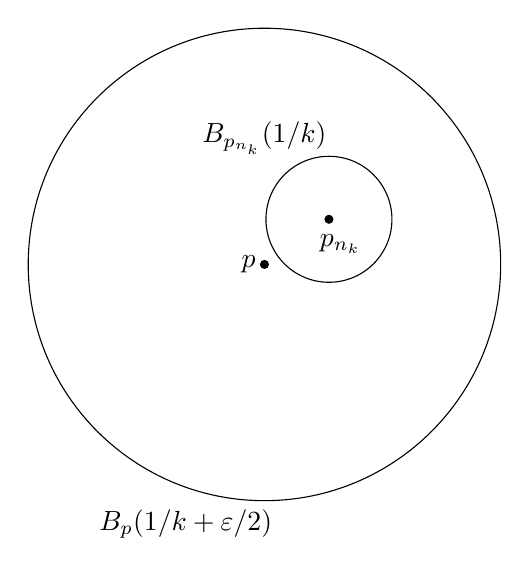
\begin{tikzpicture}
  \draw (0, 0)
  circle (3);
  \draw[fill=black] (0, 0)
  circle (0.05);
  \node at (-0.2, 0) {$p$};
  \node at (-1, -3.3) {$B_p(1/k + \varepsilon/2)$};
  \draw[fill=black] (35:1) circle
    (0.05);
  \draw (35:1) circle (0.8);
  \node at (15:1) {$p_{n_k}$};
  \node at (90:1.6) 
    {$B_{p_{n_k}}(1/k)$};
    



\end{tikzpicture}
\end{document}
